\documentclass[11pt]{article}
\usepackage[a4paper, total={6in, 8in}]{geometry}
\usepackage[utf8]{inputenc}
\usepackage[cjk]{kotex}
\usepackage{microtype}
\usepackage{hyperref}
\usepackage{listings}
\usepackage{tikz}

\renewcommand{\abstractname}{서론}

\DeclareFontFamily{\encodingdefault}{\ttdefault}{\hyphenchar\font=`\-}

\lstdefinestyle{gdb}{
    basicstyle=\ttfamily\footnotesize,
    breakatwhitespace=true,
    breaklines=true,
    frame=single
}

\usetikzlibrary{shapes.geometric, arrows}
\tikzstyle{process} = [rectangle, minimum width=3cm, minimum height=1cm, text centered, draw=black, line width=1]
\tikzstyle{arrow} = [thick, draw=gray, line width=2, ->, >=stealth]

\title{\textbf{Redis의 구조와 원리}}
\author{20201133 문해찬, 20222307 고경원, 20222327 이상명}
\date{2023년 2학기 HNU CE 임베디드시스템및실습}

\begin{document}
\sloppy
\twocolumn
\hbadness=99999
\maketitle

\begin{abstract}
Redis는 Key-Value 기반의 In-Memory 데이터베이스로서, MySQL 및 PostgreSQL과 같은
기존의 기술과 달리 하드 디스크나 SSD 등의 보조기억장치와 동기화하지 않고 단지
주기억장치만을 사용하여 임시적인 데이터를 고속으로 입출력할 수 있다. 이러한 구조 덕분에
Redis는 저장된 데이터를 빠르게 불러오기 위한 캐시나, 연계 서비스 간의 실시간 통신을
위한 메시징 시스템 등 다양한 목적으로 여러 분야에서 활용되고 있다.
\end{abstract}

\section{Redis 소스 코드의 구성}
Redis 소스 코드의 MakeFile 타깃은 서버와 CLI 및 보조 유틸리티들로 구성된다. 서버는
클라이언트로부터 전송된 요청을 수행한 후 응답하며, CLI는 단순한 클라이언트로서 사용자가
입력한 명령을 서버에 전송하고 응답을 받아온다. 또한 서버와 CLI가 지원하는 명령의
이름과 설명 및 구문 등의 명세는 JSON 포맷으로 지정되어 있으며, 파이썬 유틸리티
\texttt{generate-command-code.py}를 실행하여 실제 소스 코드
\texttt{commands.def}를 생성할 수 있다.

\section{I/O 처리 방식과 종류}
현대적인 OS의 커널이 로컬 파일, 네트워크 소켓, 인터럽트 시그널 등에 대한 핸들러 혹은
파일 디스크립터(FD)의 입출력(I/O)을 처리하는 방식은 대략 3가지 종류가 있다.

\subsection{블로킹 (동기)}
블로킹은 가장 기본적인 I/O 처리 방식으로서, 입력 혹은 출력이 완전히 완료될 때까지
무한정 대기한다. 이 방식은 I/O를 대기하는 동안 해당 프로세스가 자원을 소모하지 않으나,
다중 I/O에 대한 처리가 사실상 불가능하다.

\subsection{논-블로킹}
논-블로킹은 블로킹 방식과 달리, 입력 혹은 출력이 완료되지 않더라도 대기하지 않고 즉시
종료한다. 이 방식은 다중 I/O에 대한 처리가 가능하긴 하나, 지속적으로 I/O 처리를
시도해야 하여 자원이 상당히 많이 소모된다.

\subsection{비동기}
비동기는 블로킹과 논-블로킹을 개선한 I/O 처리 방식이다. 여러 I/O 대상들을 감시하도록
커널에 요청한 다음 대기하며, 해당 대상에 특정 이벤트가 발생하였을 경우 대기 상태를
종료하고 해당 이벤트를 즉시 처리할 수 있다. 이 방식을 사용하기 위해선 OS에서 제공하는
I/O 멀티플렉서의 API를 사용해야 한다. 대표적으로 윈도우의 IOCP, 리눅스의 Epoll,
FreeBSD 및 macOS의 Kqueue 등이 있다.

\section{Redis 서버의 이벤트 루프}
Redis 서버의 이벤트 루프는 I/O 멀티플렉서의 추상화를 담당하는 \texttt{ae.c}
라이브러리를 사용한다. 이는 Linux, FreeBSD, macOS 등 다양한 POSIX 기반 OS를
지원하며, 각 플랫폼에 맞는 효율적인 방법으로 이벤트 루프를 처리할 수 있다.
\texttt{aeMain()} 함수를 중점으로 Redis 서버의 이벤트 루프에 대해 알아본다.

\vspace{.2in}
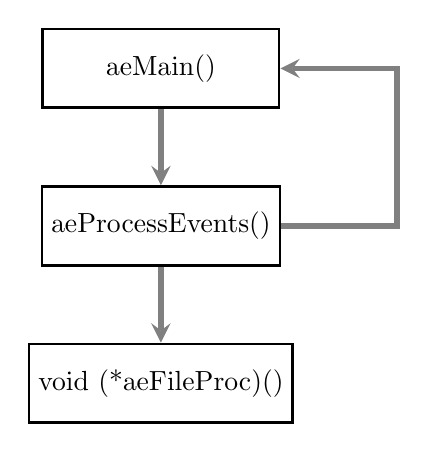
\begin{tikzpicture}[node distance=2cm]
\node (aeMain) [process]{aeMain()};
\node (aeProcessEvents) [process, below of=aeMain]{aeProcessEvents()};
\node (aeFileProc) [process, below of=aeProcessEvents]{void (*aeFileProc)()};
\draw [arrow] (aeMain) -- (aeProcessEvents);
\draw [arrow] (aeProcessEvents) -- (aeFileProc);
\draw [arrow] (aeProcessEvents) -- ++ (3cm, 0) |- node[anchor=east]{} (aeMain);
\end{tikzpicture}
\vspace{.2in}

\subsection{aeMain()}
\texttt{aeMain()} 함수는 \texttt{aeEventLoop} 구조체의 포인터를 매개변수로 받은
후, 해당 이벤트 루프의 상태를 초기화하고 무한 반복문 내부에서
\texttt{aeProcessEvents()} 함수를 호출하여 처리를 시작한다.

\subsection{aeProcessEvents()}
\texttt{aeProcessEvents()} 함수는 실제로 이벤트 루프를 처리한다.
\texttt{aeApiPoll()} 함수를 통해 커널이 감지한 이벤트의 FD를 I/O 멀티플렉서로부터
가져온 뒤, 이벤트 루프에 등록된 해당 FD의 핸들러 함수 포인터
\texttt{void (*aeFileProc)()}를 호출한다. 마지막으로 현재 처리된 이벤트의 갯수를
반환하고 종료된다.

\section{Redis 서버의 명령 처리}
Redis 서버와 CLI는 TCP 소켓 통신을 통해 요청을 주고받는다. CLI는 사용자가 쉘에
입력한 명령의 도움말을 표시하고, 해당 명령의 평문 문자열을 서버로 전송하는 사실상의
텔넷 클라이언트이다. 반면 서버는 CLI가 전송한 명령을 파싱하고 실제로 처리하는 역할을
한다. Redis 서버가 문자열 데이터를 데이터베이스에 삽입하는 명령에 대한 처리 과정은
다음과 같다.

\vspace{.2in}
\begin{lstlisting}[style=gdb]
(gdb) backtrace
#0  setGenericCommand at t_string.c
#1  setCommand at t_string.c
#2  call at server.c
#3  processCommand at server.c
#4  processCommandAndResetClient at networking.c
#5  processInputBuffer at networking.c
#6  readQueryFromClient at networking.c
#7  callHandler at connhelpers.h
#8  connSocketEventHandler at socket.c
#9  aeProcessEvents at ae.c
#10 aeProcessEvents at ae.c
#11 aeMain at ae.c
#12 main at server.c
\end{lstlisting}
\vspace{.2in}

\subsection{이벤트 루프에서 소켓 이벤트 감시}
\texttt{ae.c} 라이브러리의 이벤트 루프에서 TCP 클라이언트 소켓의 FD에 대한 이벤트를
감시한다. 이벤트가 발생한 FD가 있으면, 해당 FD의 핸들러 함수 포인터를 호출한다.

\subsection{클라이언트 소켓의 요청 수신}
클라이언트 소켓의 핸들러인 \texttt{connSocketEventHandler()}는 각 이벤트의 종류에
따른 개별적인 핸들러의 함수 포인터를 \texttt{callHandler()}를 통해 호출한다.
클라이언트 요청 수신 핸들러인 \texttt{readQueryFromClient()} 에서는 실제로 해당
소켓을 읽어들인 뒤, 요청받은 명령의 문자열을 토큰화하고 파싱한다.

\subsection{요청받은 명령 처리}
\texttt{processCommandAndResetClient()} 함수에서는
\texttt{processCommand()}를 통해 문자열 타입 API인 \texttt{t\_string.c}의
\texttt{setCommand()}를 호출한다. 이후 \texttt{resetClient()}를 호출하여 현재
요청을 처리하면서 할당되어진 메모리를 정리한다.

\subsection{데이터 타입 API 처리}
\texttt{t\_string.c}의 \texttt{setCommand()} 함수에서는
\texttt{setGenericCommand()}를 통해 문자열 데이터 타입을 처리한다.
\texttt{lookupKeyWrite()}를 통해 Key-Value 데이터베이스에서 기존의 키를 찾거나
새로 생성하고, \texttt{setKey()}를 호출하여 해당 키에 대한 값을 요청한 문자열로
지정한다.

\section{Key-Value 딕셔너리 구조}
Redis의 Key-Value 데이터베이스는 해시테이블 기반의 딕셔너리 자료구조를 사용한다.
Hiredis 라이브러리의 \texttt{dict.c} 소스에 자료구조가 구현되어 있으며,
\texttt{dictCreate()}, \texttt{dictExpand()}, \texttt{dictAdd()},
\texttt{dictFind()} 등의 API를 제공한다. \texttt{db.c}는 이 API를 사용하여
Redis의 데이터베이스를 구성한다. 해시테이블 자료구조는 해시 알고리즘을 통해 키의 고유
값을 생성하고, 이 값을 테이블의 최대 인덱스 범위로 나누어서 개별 키의 인덱스 번호를
도출한다. 이를 통해 임의의 키를 참조할 경우 $O(1)$ 이내로 접근이 가능하도록 한다.

\section{String 및 List의 자료구조}

\subsection{t\_string.c}
\texttt{t\_string.c} 데이터 타입은 힙 포인터를 사용하는 단순 C-Style 문자열이다.
\texttt{sds.c} 소스에서 이 데이터 타입을 생성하거나 복사하는 등의 간단한 조작을 할 수
있는 API를 제공한다.

\subsection{t\_list.c}
\texttt{t\_list.c} 데이터 타입은 Hiredis 라이브러리의 \texttt{quicklist.c}에서
구현된 퀵 리스트와 리스트 팩을 사용한다. 먼저 퀵 리스트는 Redis를 개발하며 고안된
자료구조인데, 링크드 리스트의 각 노드를 데이터 타입에 따라 다르게 압축하여 보관하는
자료구조인 집 리스트의 연속으로 이루어져 있다. 이를 통해 수많은 인덱스를 가진 대용량
리스트를 하나씩 순회하지 않고도, 상당히 빠른 속도로 접근이 가능하다. 하지만 저용량
리스트의 경우, 복잡한 퀵 리스트 대신 리스트 팩을 사용한다. 리스트 팩은 집 리스트를
개선한 자료구조인데, 특정 노드의 값이 변경될 경우 다른 노드까지 수정해야 하는
집 리스트의 단점을 해결하였다.

\section{작업물 URL}
\begin{enumerate}
    \item Redis 소스 코드 수정: \url{https://github.com/AIRTAG-ADV/redis}
    \item Redis 보고서 \LaTeX: \url{https://github.com/AIRTAG-ADV/redis-report}
\end{enumerate}

\end{document}
